
\chapter{Telecommunications}\label{3}


TODO: Introduction

\section{Data}
The data exchanged between a satellite and the ground stations on Earth can be divided into three different categories: the beacon, the telemetry and the telecommands.

\subsection{Beacon}

A \emph{beacon} is a radio signal transmitted continuously or periodically over a specified radio frequency. It provides a small amount of information such as identification or location, but it can have more applications. Examples of these are: adjust the power of the ground station signal based on the beacon's strength or tune the ground station to compensate the doppler shift.

\subsection{Telemetry}

\emph{Telemetry} data is sent from the satellite to the ground station and can also be divided in three sub-categories.\\

The \emph{housekeeping data} provides information abouth the health and operating status of the satellite. Examples of this data can be pressure, voltages and currents, or also bits representing the operational status of all the components as it is shown in Figure \ref{f3.1}. The size of this data is usually quite small, so a bit rate on only a few hundres of bits per second is enough to complete the transmission successfully.

\begin{figure}[H]
\centerline{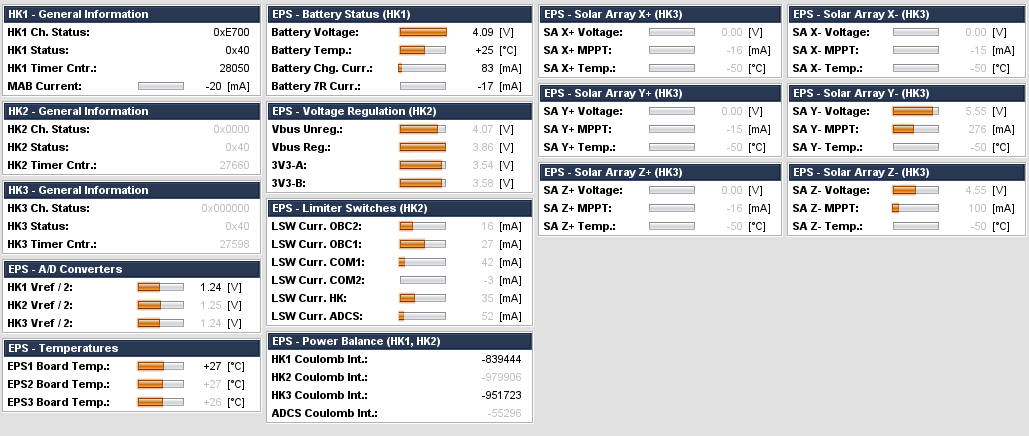
\includegraphics[width=1\textwidth]{images/housekeeping.png}}
\caption{Housekeeping data of the satellite Masat-1}
\label{f3.1}
\end{figure}

\emph{Attitude data} is generated by different sensors, such as magnetometers, gyroscopes, accelerometers and Sun, Earth and star sensors.\\

\emph{Payload data} changes with every mission and needs to be considered individually. Scientific or Earth-observing mission normally generate very large data volumes, specially in the form of images. An example of this can be Figure \ref{f3.2}, the first picture taken by the Hungarian nanosatellite Masat-1\cite{Masat}.

\begin{figure}[H]
\centerline{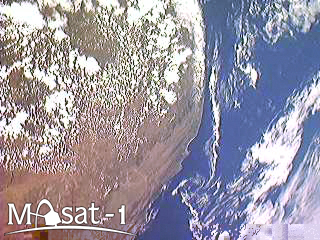
\includegraphics[width=0.7\textwidth]{images/masat.jpg}}
\caption{Picture of South Africa taken from the nanosatellite Masat-1}
\label{f3.2}
\end{figure}
\pagebreak

\subsection{Telecomands}
The telecommands are sent from the ground station to the satellite. They are used to remotely control its functions and are divided in three basic types \cite{SSEng}:
\begin{itemize}
\item \emph{Low-level on-off commands}. These are logic-level pulses used to set or reset log flip-flops.
\item \emph{High-level on-off commands}. Higher-powered pulses, capable of operating a latching relay or RF waveguide switch direcly.
\item \emph{Proportional commands}. Digital words. Used for purposes such as reprogramming memory locations on the on-board computer or setting up registers in the attitude control subsystem.

\end{itemize}

\section{Ground Station}
One integral part of every satellite mission is the ground station. It works as the first and final piece of the communication link. Its main functions are the following:
\begin{itemize}
\item Tracking the satellite to determine its position in orbit.
\item Gather data to keep track of the satellite's data and status.
\item Command operations to control the different functions of the satellite.
\item Process the received engineering and scientific data to present it in the required formats.
\end{itemize}

It is important to remember that university satellites are usually classified as amateur satellites. This means that they use amateur radio frequencies and the usage of the ground station is bound to each country's amateur radio regulations.

\subsection{Hardware}

The main components of a ground station are the antenna, the transceiver, the data recorders and the computers and their peripherals.

\subsubsection{Antennas}
The main hardware component of a ground station is the antenna. Its functions may include tracking, receiving telemetry, sending telecommands, etc.
\pagebreak

The frequencies most commonly used for amateur satellites are shown in Table \ref{Table3.1}.

\begin{table}[h]

\caption{TODO: Table with Frequencies.}
  \label{Table3.1}
\end{table}
\subsubsection{Transceiver}
A transceiver is a hardware unit containing both a transmitter and a receiver. It acts as an intermediary between the antenna and a computer, changing the radio frequency into bytes and viceversa.

\subsection{Software}
The activity in the ground station does not start when the satellite is passing over it and does not end once it is gone. There are certain tasks that need to be done before, during and after the pass.\\

Before the satellite arrives it is necessary to determine and predict its orbit. Based on this prediction the software will schedule future passes and generate the command list which will be sent during the pass.\\

The real-time software comes into operation when the satellite is visible from the ground station. It is in charge of controlling the antenna rotor to follow it across the sky; it will also send telecommands to the satellite and verify their correct reception. In addition, it will receive the data being transmitted from the satellite, which will be processed later.\\

Once the satellite is not visible any more the post-pass software comes into play. The data received during the pass is now processed and stored so the specialists can analyse it.

\subsection{Protocols}
A protocol is an agreement between the communicating parties on how communication is to proceed\cite{Tanenbaum}. This section will be focused on the OSI Reference model as well as on some of the most popular protocols for amateur radio communications.
\pagebreak
\subsubsection{The OSI Reference Model}
The Open Systems Interconnection (OSI) Reference Model was developed in 1983 and revised in 1995. This model deals with connecting systems that are open for communication with other systems. It consists on seven layers which are explained in Table 3.2.\\

\begin{table}[h]
\centering
\begin{tabular}{|l|l|l|l|}
\hline
\multicolumn{4}{|c|}{\textbf{OSI Model}}\\
\hline
& \textbf{Data Unit} & \textbf{Layer} & \textbf{Function}\\
\hline
\multirow{4}{*}{Host Layers} & \multirow{3}{*}{Data} & 7. Application & Network process to application.\\
\cline{3-4}
& & 6. Presentation & \begin{tabular}[x]{@{}l@{}}Data representation, encryption\\and decryption, convert machine\\dependent data to machine\\independent data\end{tabular}\\
\cline{3-4}
& & 5. Session &\begin{tabular}[x]{@{}l@{}}Interhost communication,\\managing sessions between\\applications\end{tabular}\\
\cline{2-4}
& Segments & 4. Transport & \begin{tabular}[x]{@{}l@{}}End-to-end connection,\\reliability and flow control\end{tabular}\\
\hline
\multirow{3}{*}{Media Layers} & Packet/Datagram & 3. Network & \begin{tabular}[x]{@{}l@{}}Path determination and\\logical adressing\end{tabular}\\
\cline{2-4}
& Frame & 2. Data link & Physical addressing\\
\cline{2-4}
& Bit & 1.Physical & \begin{tabular}[x]{@{}l@{}}Media, signal and\\binary transmission\end{tabular}\\
\hline
\end{tabular}
\caption{OSI Model\cite{Tanenbaum}.}
  \label{Table3.2}
\end{table}

\pagebreak

\subsubsection{AX.25}
AX.25 is a data link layer protocol designed for use by amateur radio operators. It occupies the first, second and third layers of the OSI model. However, AX.25 was developed before the model came into action, so its specification was no written to separate into OSI layers.\\

The link-layer packet radio transmission takes place in small blocks of data called frames. Those frames are represented in the Figures \ref{f3.3} and \ref{f3.4}.\\

 \begin{figure}[H]
\centerline{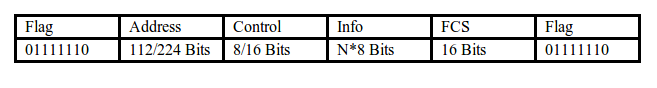
\includegraphics[width=1\textwidth]{images/ax25a.png}}
\caption{Supervisory and Unnumbered frames \cite{AX25}}
\label{f3.3}
\end{figure}

\begin{figure}[H]
\centerline{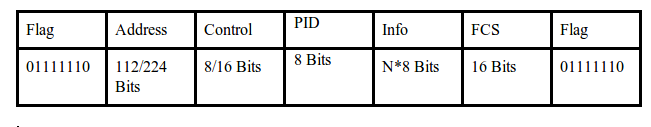
\includegraphics[width=1\textwidth]{images/ax25b.png}}
\caption{AX.25 Information frame \cite{AX25}}
\label{f3.4}
\end{figure}

\subsubsection{FX.25}
FX.25 is an extension to the AX.25 protocol. It has been created to complement the AX.25 protocol, providing an encapsulation mechanism that does not alter the AX.25 data or functionalities. AX.25 packets are easily damaged, and this extension intends to remedy the situation by providing a Forward Error Correction (FEC) capability at the bottom of Layer 2.

\begin{figure}[H]
\centerline{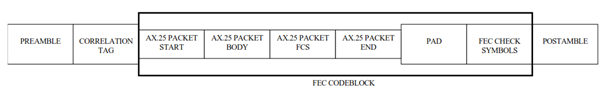
\includegraphics[width=1\textwidth]{images/fx25.png}}
\caption{AX.25 Information frame \cite{FX25}}
\label{f3.5}
\end{figure}

\newpage